\section{Microarchitecture}

Coarse grain execution exposes energy saving opportunities in most pipeline
stages. In this section we discuss the flow of basicblocks through different
pipeline stages and elaborate on how energy is saved in each stage.

Figure~\ref{fig:bb_arch} and~\ref{fig:pipeline} show the basic-block execution
flow through the BBE pipeline and the BBE micro-architecture. The hardware units
distinguishing BBE from OoO are the Basic-block Windows (BB Window), Local Register
File (LRF), Basic-block Re-order Buffer (BB-ROB), the Register Rename bypass
line, basic-block scheduler, and the branch Prediction lookup line coming 
from the BB Scheduler rather than instruction fetch.

\begin{figure*}
	\centering
	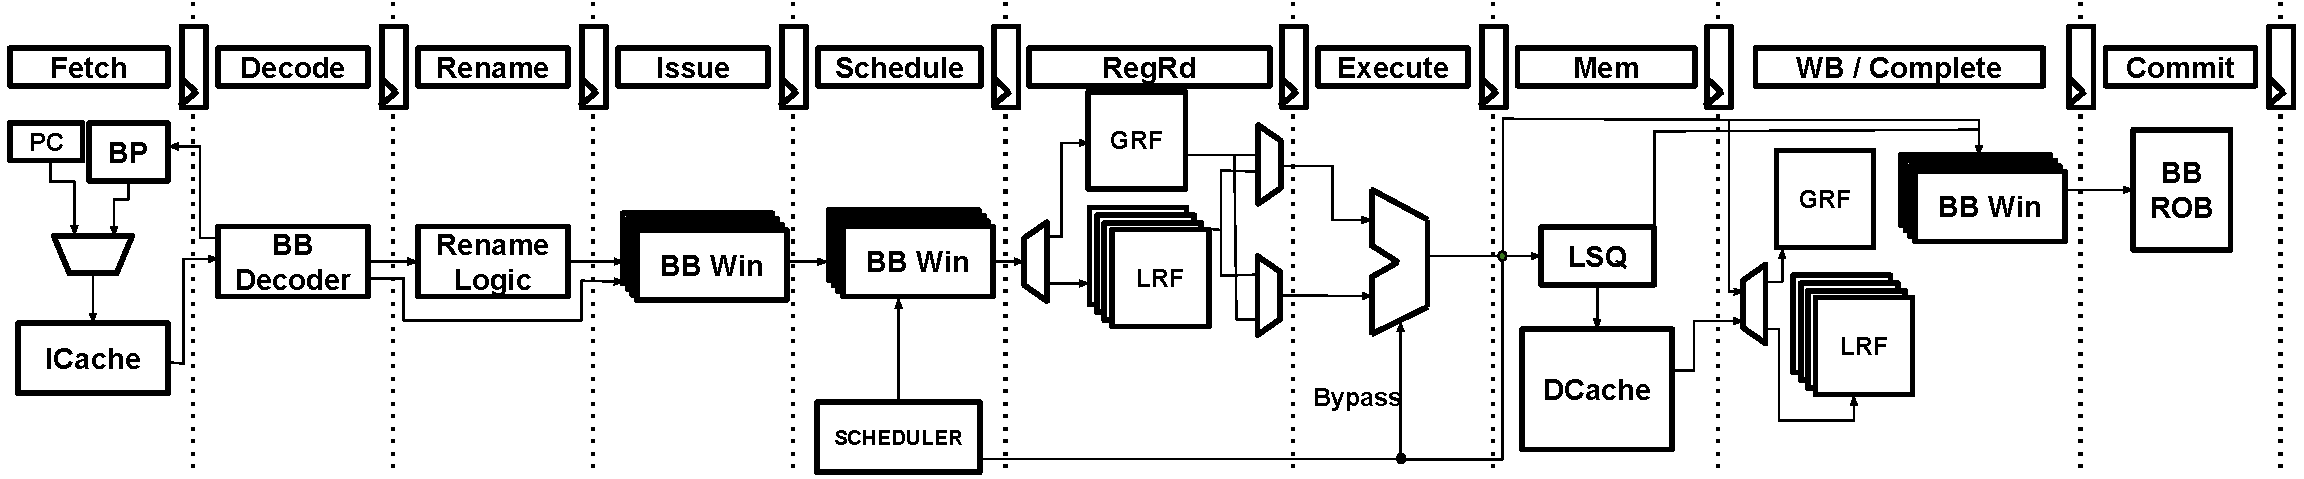
\includegraphics[width=\textwidth]{fig/pipeline.pdf} 
	\caption{Basicblock execution pipeline}
	\label{fig:pipeline}
\end{figure*}

\begin{figure}
	\centering
	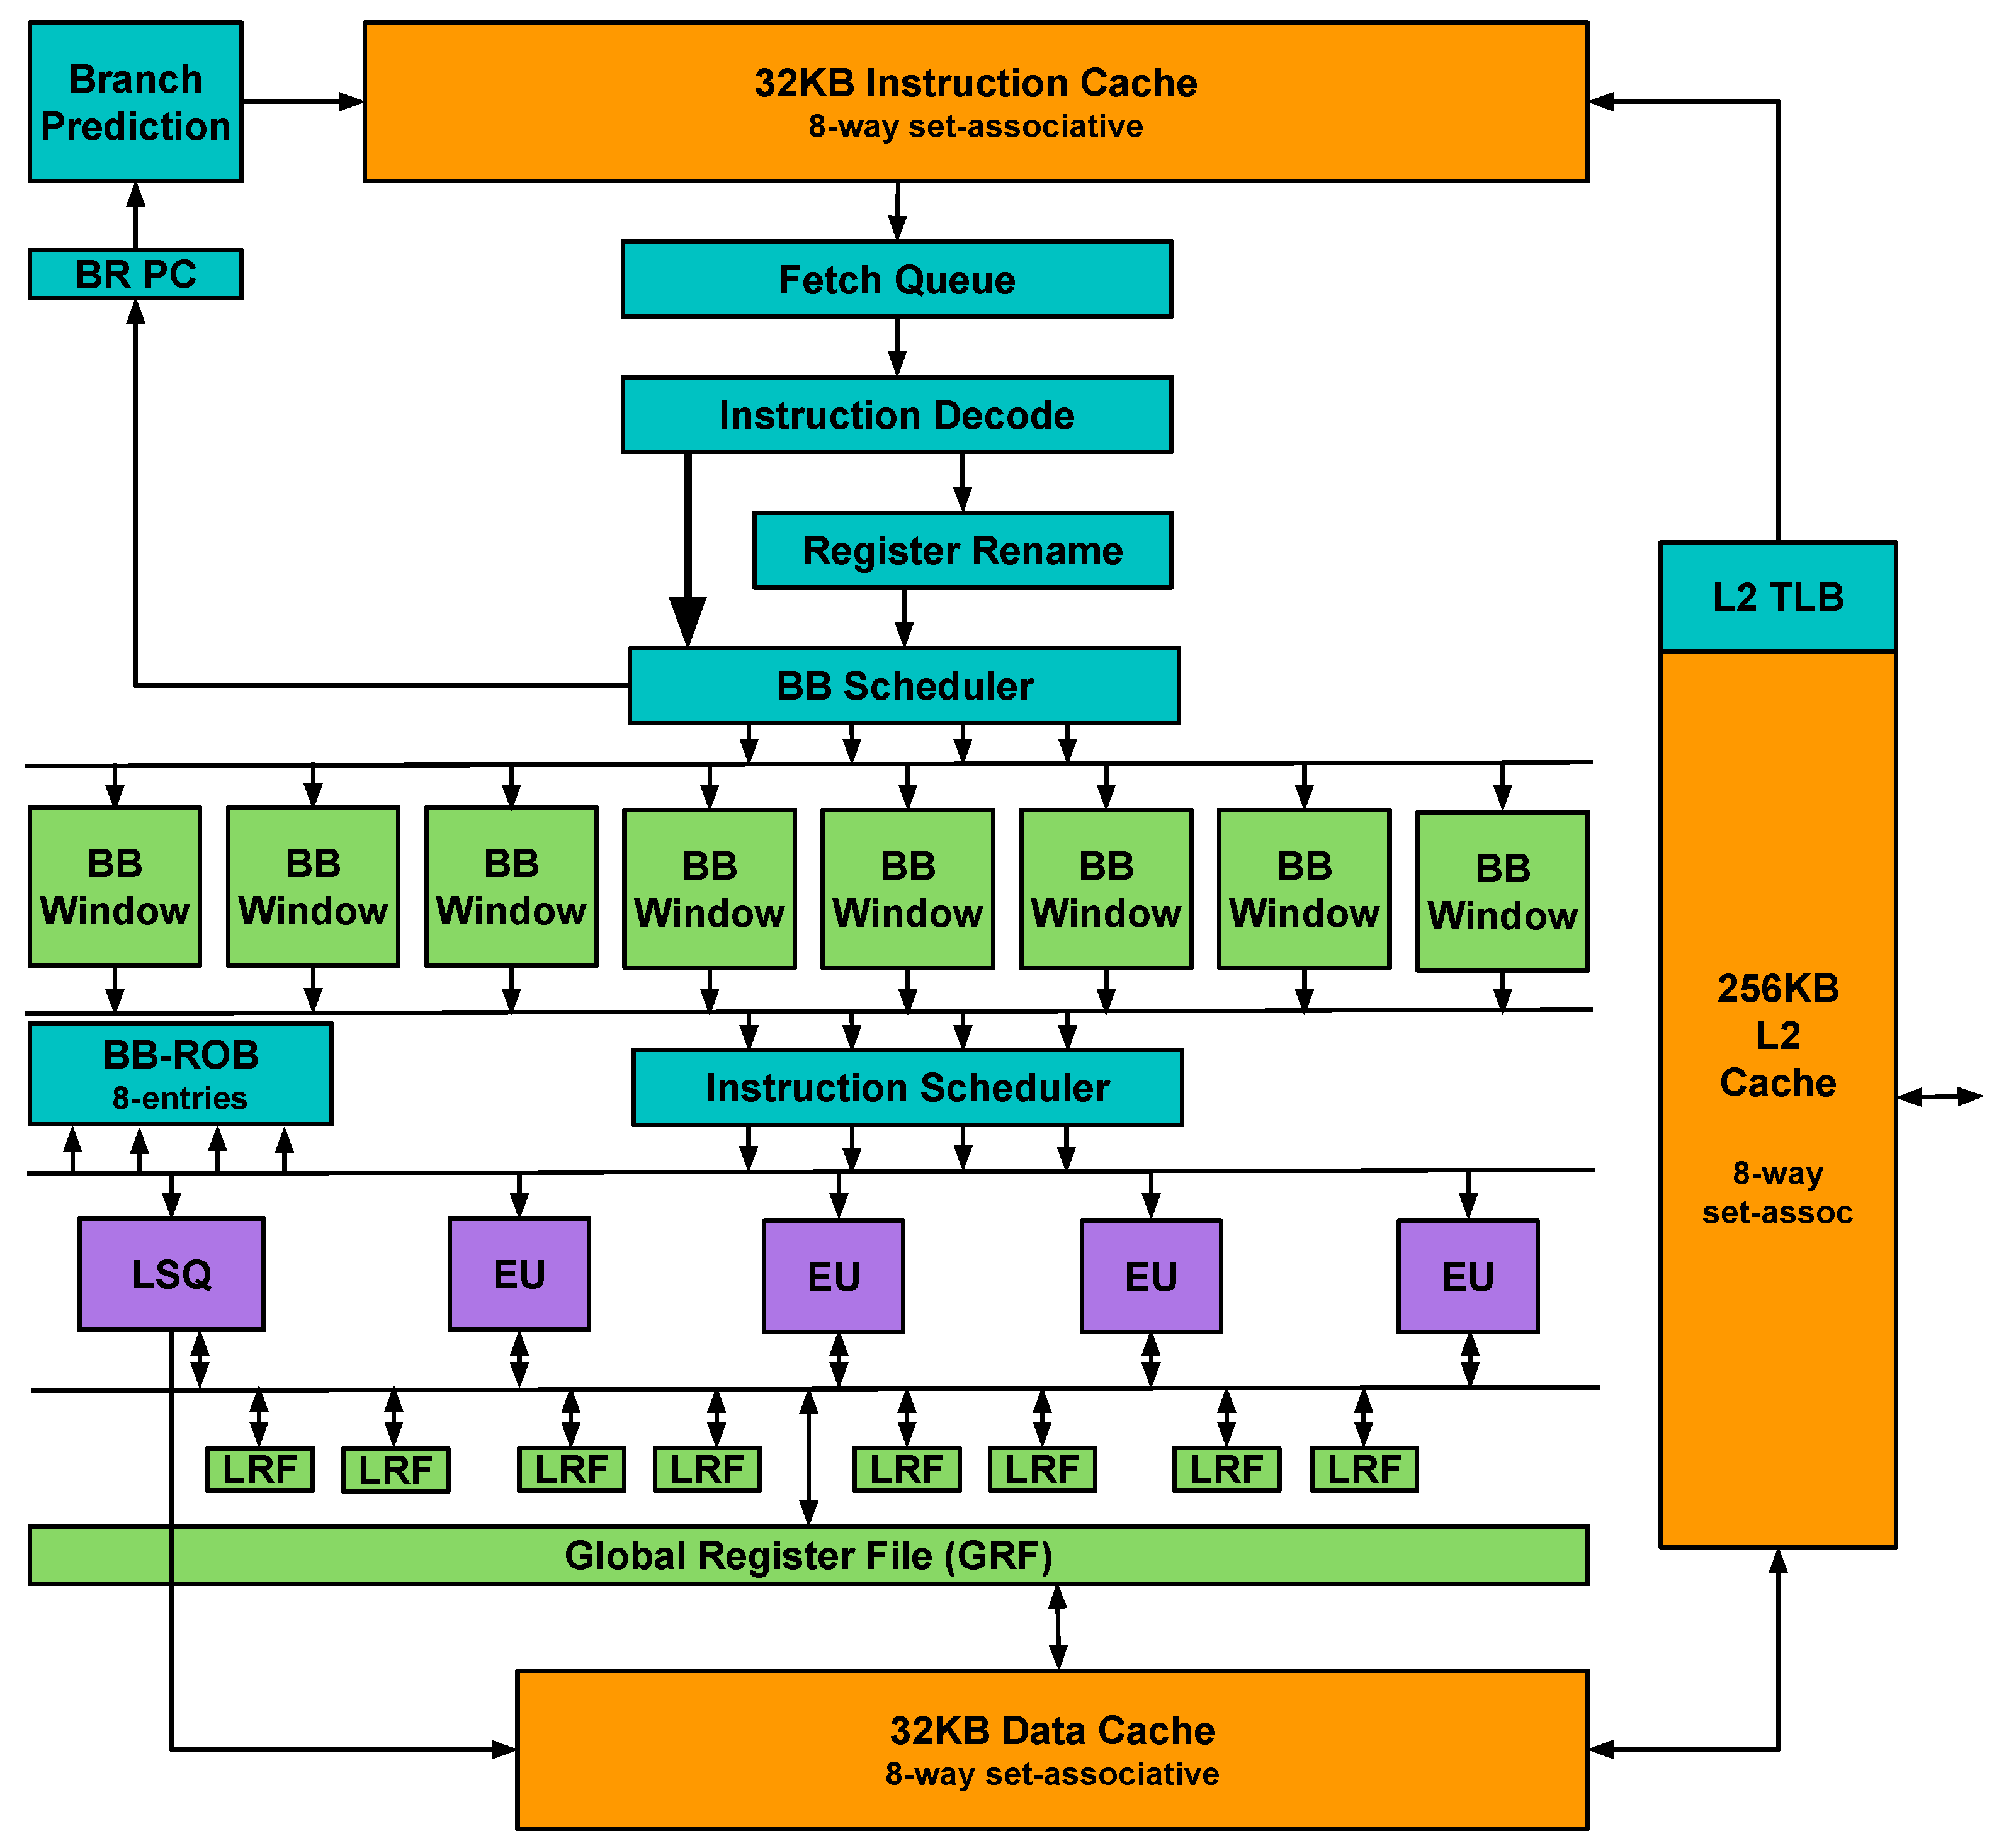
\includegraphics[width=1.0\columnwidth]{fig/bb_architecture.pdf} 
	\caption{Basicblock execution microarchitecture}
	\label{fig:bb_arch}
\end{figure}

\subsection{CPU Frontend}
\label{sec:cpu_frontend}

discussion of register renaming and branch prediction lookup and update models.

% The processor frontend consists of the branch-prediction, fetch, decode, and
% register rename stages. Branch prediction only looks up H instructions. Fetch
% and decode stages are designed similar to existing architectures with
% configurable withs of 2, 4, 8. Contrary to the OoO model where register renaming
% happens in dispatch stage, here register renaming is done right after decode
% (explain why).  The register rename unit is only accessed by H instructions.
% Local registers do not access the register rename unit.
% 
% Given the smaller utility of register renaming, this processor can use a
% smaller set of physical registers (less area and energy per access).


\subsection{CPU Backend}
\label{sec:cpu_backend}

The backend consists of several basicblock window buffers used to store
basicblock operations and the meta-data associated with each BB, local registers
for each basicblock, a global register file, execution units, basicblock reorder
buffer (BBROB), a load-store queue model, and the wake-up logic.

%\subsubsection{Basicblock Window}
\label{sec:bb_window}

\textbf{BB Windows} are FIFO buffers used to store up to 16 outstanding
instructions.  Instructions in a BB Window execute in-order. In
Figure~\ref{fig:bb_arch}, eight BB Windows are shown where each BB Window can
issue up to two instructions per cycle. Each cycle, the head of each BB Window
is checked for ready instruction(s). If more than four instructions are
available, the four oldest instructions are issued. Since BB Windows are FIFO
structures, we find their lookup and update energy overhead is an order of
magnitude smaller than reservation station tables.
%justify hwy two instructions

\begin{figure}
	\centering
	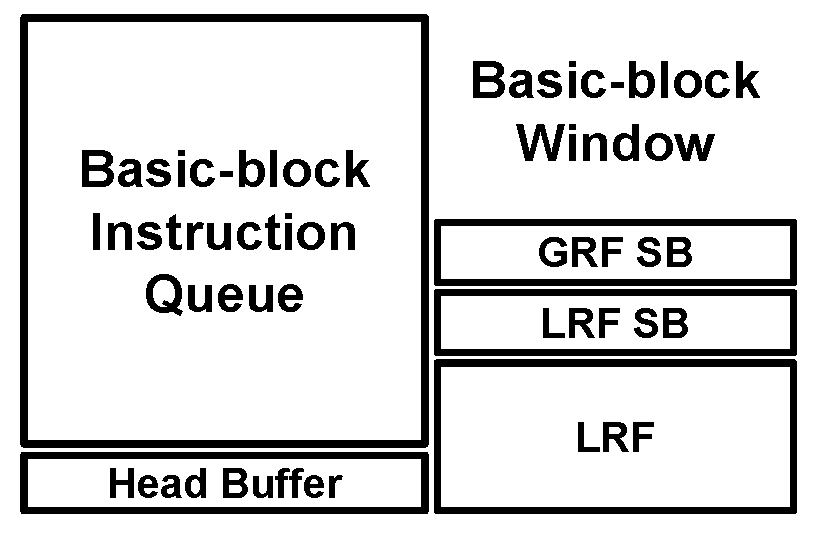
\includegraphics[width=0.6\columnwidth]{fig/bb_window.pdf} 
	\caption{Basicblock window structure}
	\label{fig:bb_window}
\end{figure}

\textbf{LRF} is a simple register file with at most 8 statically
allocated register elements. Each BB Window has its own dedicated basic-block
that is used to support storing register entries that are live only within the
basic-block lifetime. Once the basic-block completes its execution, the content
of these LRF's are invalidated. Figure~\ref{fig:bb_window} illustrates the hardware
elements supporting BB Window. GRF SB and LRF SB are the scoreboard tables used
to store the basic-block global read. A LRF SB entry is made valid once its
corresponding write operands updates the LRF. A GRF SB entry is also updated
when a global operands is about to write its valud to the GRF; the difference is a
global operand broadcasts to all GRF SB's. Since GRF SB's are small CAM arrays
with at most 7 global entries, the energy overhead of updating them is
negligible compared to an instruction window broadcast update.

Head Buffer in Figure~\ref{fig:bb_window} holds the instruction(s) pending to be
issued from the BB Window.

Figure XX shows the average number of in-flight basicblocks for SPEC2006
benchmark.

%Instructions hold offset to the instruction rather than to actual register
%address. This cuts back the register address by half (making the ISA shorter)
%    and also enable RAM lookup to the GRF table upon lookup.

%GRF scoreboard update is CAM baesd, but its lookup is RAM based. (very cheap)
%    update: CAM lookup to address ready bit
%    lookup: RAM lookup to the 1bit entry.



\subsubsection{Register File Structure}
\label{sec:reg_files}

We find that on average roughly 50\% of data communication in SPEC benchmarks
are done across def-uses that have sub-basicblock live ranges. Such registers
do not need to be register renamed if an additional register space is available
for them to temporarily hold their values for the upcoming user instruction.  As
a result, two classes of registers are defined in this architecture: local registers
and a global register. The global register is a big register file with register
renaming support. Local registers, on the other hand, are small register
file blocks with no register renaming; allocation for these registers is
done at compile time.  Global registers are designed for data communication
across basicblocks while local registers are designed for data communication
within a bsaicblock.

\subsubsection{Basicblock Reorder Buffer (BBROB)}
\label{sec:bb_rob}

Contrary to the OoO execution model where the program order is tracked at
instruction granularity through the reorder buffer (ROB), in this design, we only
track program order at basic-block granularity. BBROB is a content addressable
memory array (CAM) with only 16 entries (~10x smaller than ROB size in OoO) that
enables issuing, committing, and squashing basic-blocks as a whole in one cycle
(per basic-block). The smaller size of BBROB compared to a ROB enables
significant energy savings.

BBROB is marked complete when all its operations are completed. Complete
operands increment the completion counter in their BBROB entry. Once the counter
reaches the expected BB size, the BB is marked complete. BBE can commit up to
one BB per cycle, allowing bulk commit using one port to the table. At commit,
    the global write operands in the BB will be marked non-speculative.

%Discussion on what is held on each BBROB entry: BBID, number of completed
%basic-block instructions, total number of instructions in the BB that need to
%complete, valid bit, mis-speculation bit, global physical register writes.

%Discussion on how basic-block entry updates the GRF upon commit through its
%global physical register writes (its GRF write register(s) go from speculative
%to architectural).

%After the decode stage, a BB entry is reserved in BBROB, and when all
%instructions in a basic-block are completed and the basic-block reaches the head
%of the BBROB, the basic-block is committed as a whole in one cycle. Upon a branch
%mis-speculation event (either branch or memory), younger basic-blocks are flushed
%in one cycle. (TODO: talk more about the squash process here)



\subsection{Squash Handling}
\label{sec:speculation}

In BBE, squash events are handled at basic-block granularity. To avoid wasting
{\it{useful}} instructions executed in a mis-speculated BB, the compiler uses
profiling information to separate weakly biased branches form the rest of the BB
into a single-instruction BB. Less than XX\% of useful instructions are wasted
in BBE.

The average number of BB's squashed per mis-prediction event is 6 where each
basic-block has an average of 3 global write operands. BBE is able to invalidate
register renaming entries within 5 cycles which is comparable to the number of
cycles OoO takes to restore a checkpoint and restart the execution. This
approach eliminates the need for both program checkpointing and a second
register alias table.

% how many cycles does it take to load a checkpoint?
% how much energy is it to track checkpoints?


%Memory mis-prediction is less likely in this model as each basicblock buffer
%runs in-order (no chance of mis-speculation between load-stores within a
%basicblock). We also say that mis-speculation handling is the same for
%both memory and branch.


%provide an example of the execution here.  it should contain a code with
%multiple BB's with local/global registers, header ins.  It should show flow of
%BB in a 2-wide machine. provide execution schedule, update and issue register
%activity. instruction issue logic information.

%TODO discuss how large basicblocks are partitioned.
%TODO Talk about exception handling here.
%\subsection{Basicblock Scheduling}
\label{sec:scheduling}

Instruction scheduling example.

Scheduling consists of:

1) ready check: find ready instructions from head of BB - what are the
dependency checks done?

2) update check: blast write operands to all BB-header buffers. 

3) discussion of available bbWindow detection and bbWidnow allocation

% This unit is broken into two main sub-units: instruction issue and instruction
% update. The instruction issue unit looks for ready instructions at the
% head of each basicblock window buffer on every cycle. The instruction udpate
% unit updates global and local register values.
% 
% Update unit discussion goes here. It talks about updating local registers and
% their ready bits, and updating basicblock headers to indicate if the global
% operands of different instructions in a basicblock are ready.
% 
% Issue unit discussion goes here. It talks about how the issue unit checks the
% corresponding local and global operands of an instruction to determine if the
% instruction is ready. Global operands availability is checked by looking up the
% BB header (where the update unit marks a valid bit for each pgysical global
% operand that is ready) and the local operands are checked by lookup
% their up valid bit in the corresponding LRF. 
% 
% Here we also discuss the energy efficiency implications of looking up the head
% of 16 basicblock buffers rather than blasting through a 120 entry instruction
% window (which is a CAM array). We also discuss how basicblock headers help
% reduce the number of check-for-ready-operands accesses to GRF by keeping ready
% information for each global register value in the header of the BB.
% %TODO you need to implement this

%discussion on ISA changes
